% questions.tex —— 1956 年·全国卷 · 题目内容片段（无答案）
% 由 tools/generate_projects.py 依来源总账自 1956/1956_数学真题_试题.md 生成，勿手改（改源 MD 后重跑）


\begin{gktip}
\textbf{题面说明}：本卷原件要求考生按“一甲、一乙、二、三”等题号顺次作答。为适配可复用题库，本文将“一”中的甲、乙、丙、丁、戊及二至五统一编号为第 1—10 题；原卷中的图形在 LaTeX 成品中以 TikZ 矢量源重绘。
\end{gktip}

\gkpart{一、小题}

\begin{question}
\gkti{1}（甲）利用对数性质，计算 $(\lg 5)^2+\lg 2\cdot\lg 50$。

（注：原卷中第一个 2 为上标，表示 $(\lg 5)^2$。）

\end{question}
\begin{question}
\gkti{2}（乙）设 $m$ 是实数，求证方程
\[
2x^2-(4m-1)x-m^2-m=0
\]
的两个根必定都是实数。

\end{question}
\begin{question}
\gkti{3}（丙）设 $M$ 是 $\triangle ABC$ 的边 $AC$ 的中点，过 $M$ 作直线交 $AB$ 直线于 $E$，过 $B$ 作直线平行于 $ME$ 交 $AC$ 直线于 $F$。求证 $\triangle AEF$ 的面积等于 $\triangle ABC$ 的面积的一半。

\end{question}
\begin{question}
\gkti{4}（丁）一个三角形三边的长分别是 $3$ 尺、$4$ 尺及 $\sqrt{37}$ 尺，求这个三角形的最大角的度数。

\end{question}
\begin{question}
\gkti{5}（戊）设 $\tan\alpha$ 与 $\tan\beta$ 是方程 $x^2+6x+7=0$ 的两个根，求证
\[
\sin(\alpha+\beta)=\cos(\alpha+\beta).
\]

\end{question}
\gkpart{二、大题}

\begin{question}
\gkti{6}解联立方程
\[
\begin{cases}
7\sqrt{x+y}-x-y=12,\\
x^2+y^2=136.
\end{cases}
\]

\end{question}
\begin{question}
\gkti{7}设 $P$ 是等边三角形 $ABC$ 外接圆不含 $A$ 的小弧 $\widehat{BC}$ 上的一点，求证
\[
PA^2=AB^2+PB\cdot PC.
\]

\Needspace{0.4\textheight}
\end{question}
\begin{question}
\gkti{8}有一四棱柱体，底面 $ABCD$ 为菱形，且
$\angle A'AB=\angle A'AD$（如图），求证平面 $A'ACC'$ 垂直于底面 $ABCD$。
\nopagebreak[4]
\begin{center}% 1956 年全国卷第 8 题：底面 ABCD 为菱形的四棱柱示意图。
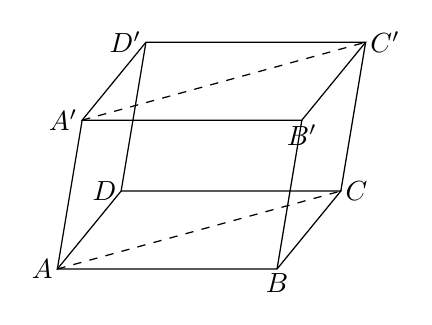
\begin{tikzpicture}[scale=0.9, line width=0.45pt,
  every node/.style={inner sep=1.5pt}]
  \coordinate (A) at (0,0);
  \coordinate (B) at (3.1,0);
  \coordinate (C) at (4.0,1.1);
  \coordinate (D) at (0.9,1.1);
  \coordinate (A1) at (0.35,2.1);
  \coordinate (B1) at (3.45,2.1);
  \coordinate (C1) at (4.35,3.2);
  \coordinate (D1) at (1.25,3.2);
  \draw (A)--(B)--(C)--(D)--cycle;
  \draw (A1)--(B1)--(C1)--(D1)--cycle;
  \draw (A)--(A1) (B)--(B1) (C)--(C1) (D)--(D1);
  \draw[dashed] (A)--(C) (A1)--(C1);
  \node[anchor=east] at (A) {$A$};
  \node[anchor=north] at (B) {$B$};
  \node[anchor=west] at (C) {$C$};
  \node[anchor=east] at (D) {$D$};
  \node[anchor=east] at (A1) {$A'$};
  \node[anchor=north] at (B1) {$B'$};
  \node[anchor=west] at (C1) {$C'$};
  \node[anchor=east] at (D1) {$D'$};
\end{tikzpicture}
\end{center}
\nopagebreak[4]
\end{question}
\begin{question}
\gkti{9}若三角形的三个角成等差级数，则其中一定有一个角是 $60^\circ$；试证明之。

\end{question}
\begin{question}
\gkti{10}若上述三角形的三边又成等比级数，则三个角都是 $60^\circ$，试证明之。

\end{question}